\section{Design and Implementation}
\label{sec:arch}

\tritonsort is a distributed, staged, pipeline-oriented dataflow processing
system. In this section, we describe \tritonsort's design and motivate our
design decisions for each stage in its processing pipeline.

\subsection{Architecture Overview}

Figures \ref{fig:phase1} and \ref{fig:phase2} show the stages of a \tritonsort
program.  See Chapter~\ref{chapter:principles} for details on how \tritonsort's
stages operate.

In the process of executing its \textit{run()} method, a worker can get buffers
from and return buffers to a shared pool of buffers.  This buffer pool can be
shared among the workers of a single stage, but is typically shared between
workers in pairs of stages with the upstream stage getting buffers from the
pool and the downstream stage putting them back.  When getting a buffer from a
pool, a stage can specify whether or not it wants to block waiting for a buffer
to become available if the pool is empty.

\subsection{Sort Architecture}

We implement sort in two phases.  First, we perform distribution sort to
partition the input data across $L$ logical partitions evenly distributed
across all nodes in the cluster.  Each logical partition is stored in
its own \emph{logical disk}.  All logical disks are of identical maximum size
$size_{LD}$ and consist of files on the local file system.

The value of $size_{LD}$ is chosen such that logical disks
from each physical disk can be read, sorted and written in parallel in the
second phase, ensuring maximum resource utilization.  Therefore, if the size of
the input data is $size_{input}$, there are $L =
\frac{size_{input}}{size_{LD}}$ logical disks in the system.  In phase two, the
records in each logical disk get sorted locally and written to an output file.
This implementation satisfies our design goal of reading and writing each record
twice.

To determine which logical disk holds which records, we logically partition the
10-byte key space into $L$ even divisions.  We logically order the logical
disks such that the $k^{th}$ logical disk holds records in the $k^{th}$
division.  Sorting each logical disk produces a collection of output files,
each of which contains sorted records in a given partition.  Hence, the ordered
collection of output files represents the sorted version of the data.  In this
paper, we assume that records' keys are distributed uniformly over the key
range which ensures that each logical disk is approximately the same size; we
discuss how to handle non-uniform key ranges in Chapter~\ref{chapter:themis}.

To ensure that we can utilize as much read/write bandwidth as possible on each
disk, we partition the disks on each node into two groups of 8 disks each. One
group of disks holds input and output files; we refer to these disks as the
input disks in phase one and as the output disks in phase two.  The other group
holds intermediate files; we refer to these disks as the intermediate disks.
In phase one, input files are read from the input disks and intermediate files
are written to the intermediate disks. In phase two, intermediate files are
read from the intermediate disks and output files are written to the output
disks. Thus, the same disk is never concurrently read from and written to,
which prevents unnecessary seeking.

\subsection{\tritonsort Architecture: Phase One}

\begin{figure*}
  \centering 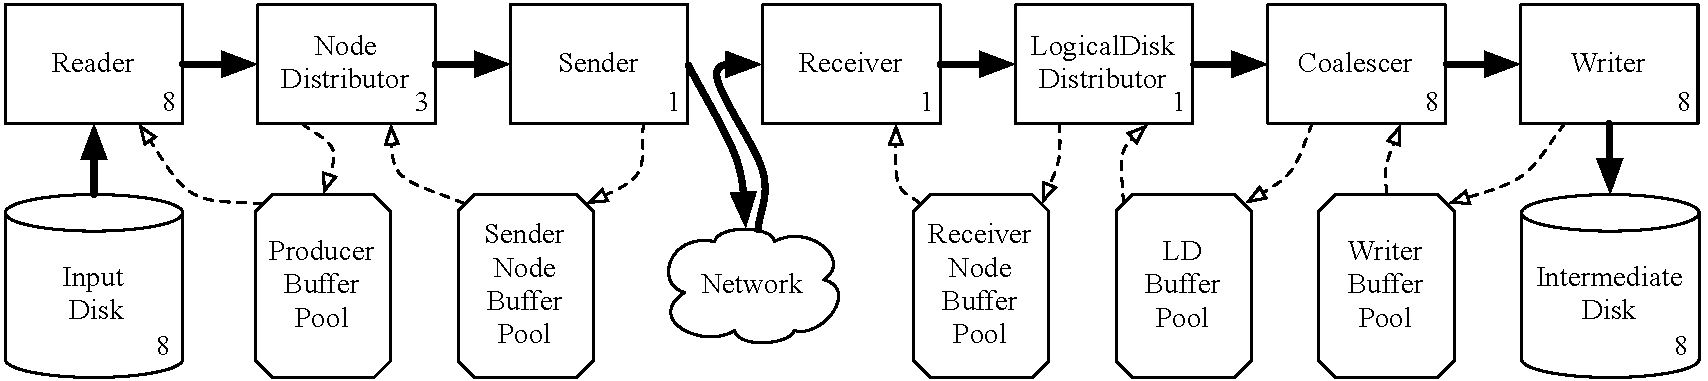
\includegraphics[width=\textwidth]{tritonsort/figs/phase1.pdf}

  \caption{Block diagram of \tritonsort's phase one architecture.  The
    number of workers for a stage is indicated in the lower-right corner of
    that stage's block, and the number of disks of each type is indicated in
    the lower-right corner of that disk's block.}

  \label{fig:phase1}
\end{figure*}

Phase one of \tritonsort, diagrammed in Figure~\ref{fig:phase1}, is responsible
for reading input records off of the input disks, distributing those records
over to the network to the nodes on which they belong, and storing them into
the logical disks in which they belong.

\paragraph{\reader:} Each \reader is assigned an input disk and
is responsible for reading input data off of that disk.  It does this by
filling 80 MB \producerbuffers with input data.
We chose this size because it is large
enough to obtain near sequential throughput from the disk.

\begin{figure}
  \centering
  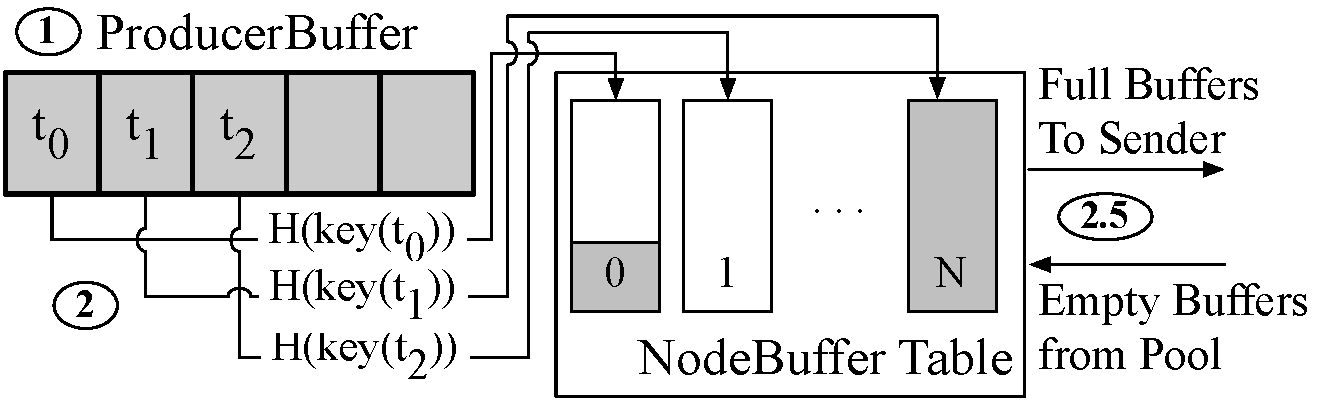
\includegraphics[width=\columnwidth]{tritonsort/figs/pnts_stage.pdf}
  \caption{The \pnts stage, responsible for partitioning records by
    destination node.}
  \label{fig:pnts}
\end{figure}

\paragraph{\pnts:} A \pnts (shown in Figure~\ref{fig:pnts}) receives a
\producerbuffer from a \reader and is responsible for partitioning the records
in that buffer across the machines in the cluster.  It maintains an internal
data structure called a \emph{\nodebuffer table}, which is an array of
\nodebuffers, one for each of the nodes in the cluster.  A \nodebuffer contains
records belonging to the same destination machine.  Its size was chosen to be
the size of the \producerbuffer divided by the number of nodes, and is
approximately 1.6 MB in size for the scales we consider in this paper.

The \pnts scans the \producerbuffer record by record.  For each record, it
computes a hash function $H(k)$ over the record's key $k$ that maps the record to
a unique host in the range $[0,N-1]$.  It uses the \nodebuffer table to select
a \nodebuffer corresponding to host $H(k)$ and appends the record to the end of
that buffer.  If that append operation causes the buffer to become full, the
\pnts removes the \nodebuffer from the \nodebuffer table and sends it
downstream to the \sender stage.  It then gets a new \nodebuffer from the
\nodebuffer pool and inserts that buffer into the newly empty slot in the
\nodebuffer table.  Once the \pnts is finished processing a
\producerbuffer, it returns that buffer back to the \producerbuffer pool.

\begin{figure}
  \centering
  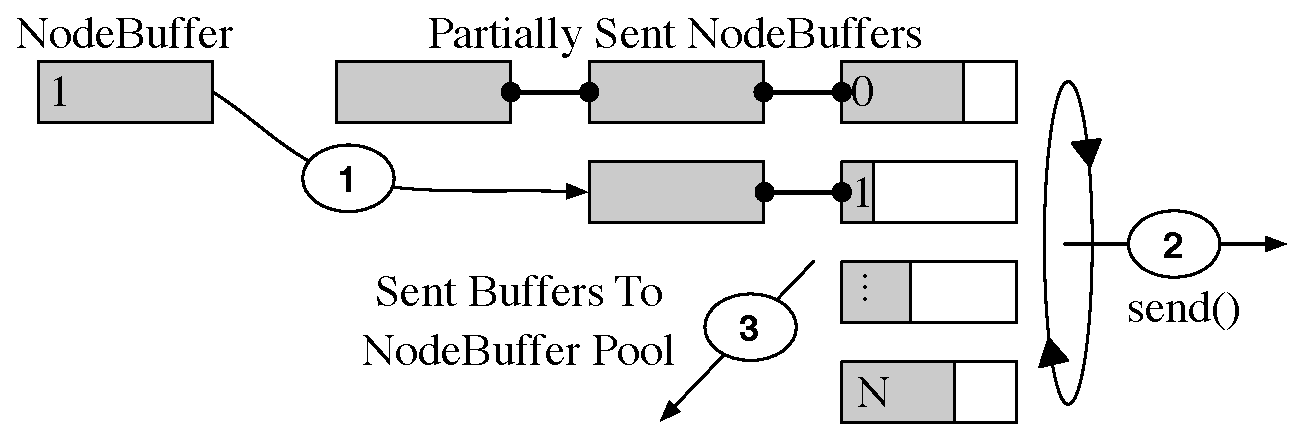
\includegraphics[width=\columnwidth]{tritonsort/figs/sender_stage.pdf}
  \caption{The \sender stage, responsible for sending data to
    other nodes.}
  \label{fig:sender}
\end{figure}

\paragraph{\sender:}  The \sender stage (shown in Figure~\ref{fig:sender}) is
responsible for taking \nodebuffers from the upstream \pnts stage and
transmitting them over the network to each of the other nodes in the cluster.
Each \sender maintains a separate TCP socket per peer node in the cluster.  The
\sender stage can be implemented in a multi-threaded or a single-threaded
manner.  In the multi-threaded case, $N$ \sender workers are instantiated in
their own threads, one for each destination node.  Each \sender worker simply
issues a blocking \textit{send()} call on each \nodebuffer it receives from the
upstream \pnts stage, sending records in the buffer to the appropriate
destination node over the socket open to that node.  When all the records in a
buffer have been sent, the \nodebuffer is returned to its pool, and the next
one is processed.  For reasons described in Section~\ref{sec:fastnetwork}, we
choose a single-threaded \sender implementation instead.  Here, the \sender
interleaves the sending of data across all the destination nodes in small
non-blocking chunks, so as to avoid the overhead of having to activate and
deactivate individual threads for each send operation to each peer.

Unlike most other stages, which process a single unit of work during each
invocation of their \textit{run()} method, the \sender continuously processes
\nodebuffers as it runs, receiving new work as it becomes available from the
\pnts stage.  This is because the \sender must remain active to alternate
between two tasks: accepting incoming \nodebuffers from upstream \pntss, and
sending data from accepted \nodebuffers downstream.  To facilitate accepting
incoming \nodebuffers, each \sender maintains a set of \nodebuffer lists, one
for each destination host.  Initially these lists are empty.  The \sender
appends each \nodebuffer it receives onto the list of \nodebuffers
corresponding to the incoming \nodebuffer's destination node.

To send data across the network, the \sender loops through the elements in the
set of \nodebuffer lists.  If the list is non-empty, the \sender accesses the
\nodebuffer at the head of the list, and sends a fixed-sized amount of data to
the appropriate destination host using a non-blocking \textit{send()} call.  If
the call succeeds and some amount of data was sent, then the \nodebuffer at the
head of the list is updated to note the amount of its contents that have been
successfully sent so far.  If the \textit{send()} call fails, because the TCP
send buffer for that socket is full, that buffer is simply skipped and the
\sender moves on to the next destination host.  When all of the data from a
particular \nodebuffer is successfully sent, the \sender returns that buffer
back to its pool.

\begin{figure}
  \centering 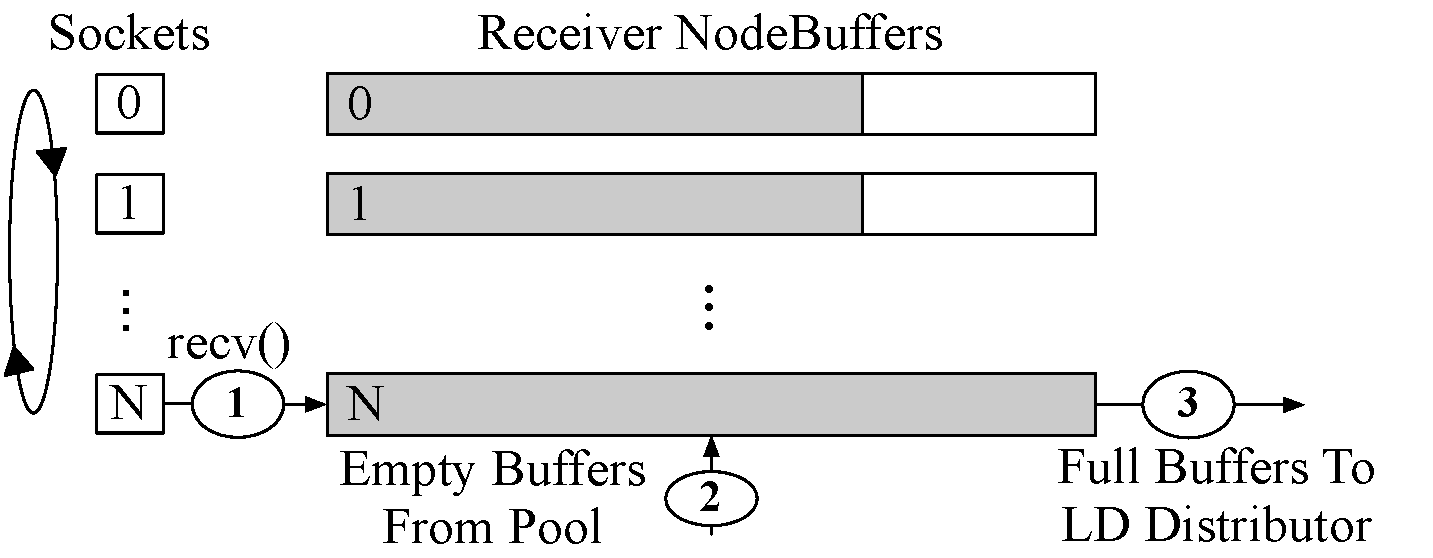
\includegraphics[width=\columnwidth]{tritonsort/figs/receiver_stage.pdf}
  \caption{The \receiver stage, responsible for receiving data from other
    nodes' \sender stages.}
  \label{fig:receiver}
\end{figure}

\paragraph{\receiver:}  The \receiver stage, shown in
Figure~\ref{fig:receiver}, is responsible for receiving data from other nodes
in the cluster, appending that data onto a set of \nodebuffers, and passing
those \nodebuffers downstream to the \ldts stage.  In \tritonsort, the
\receiver stage is instantiated with a single worker.  On starting up, the
\receiver opens a server socket and accepts incoming connections from \sender
workers on remote nodes.  Its \textit{run()} method begins by getting a set of
\nodebuffers from a pool of such buffers, one for each source node.  The
\receiver then loops through each of the open sockets, reading up to 16KB of
data at a time into the \nodebuffer for that source node using a non-blocking
\textit{recv()} call.  This small socket read size is due to the rate-limiting
fix that we explain in Section~\ref{sec:fastnetwork}.  If data is returned by
that call, it is appended to the end of the \nodebuffer.  If the append would
exceed the size of the \nodebuffer, that buffer is sent downstream to the \ldts
stage, and a new \nodebuffer is retrieved from the pool to replace the
\nodebuffer that was sent.

\begin{figure}
  \centering
  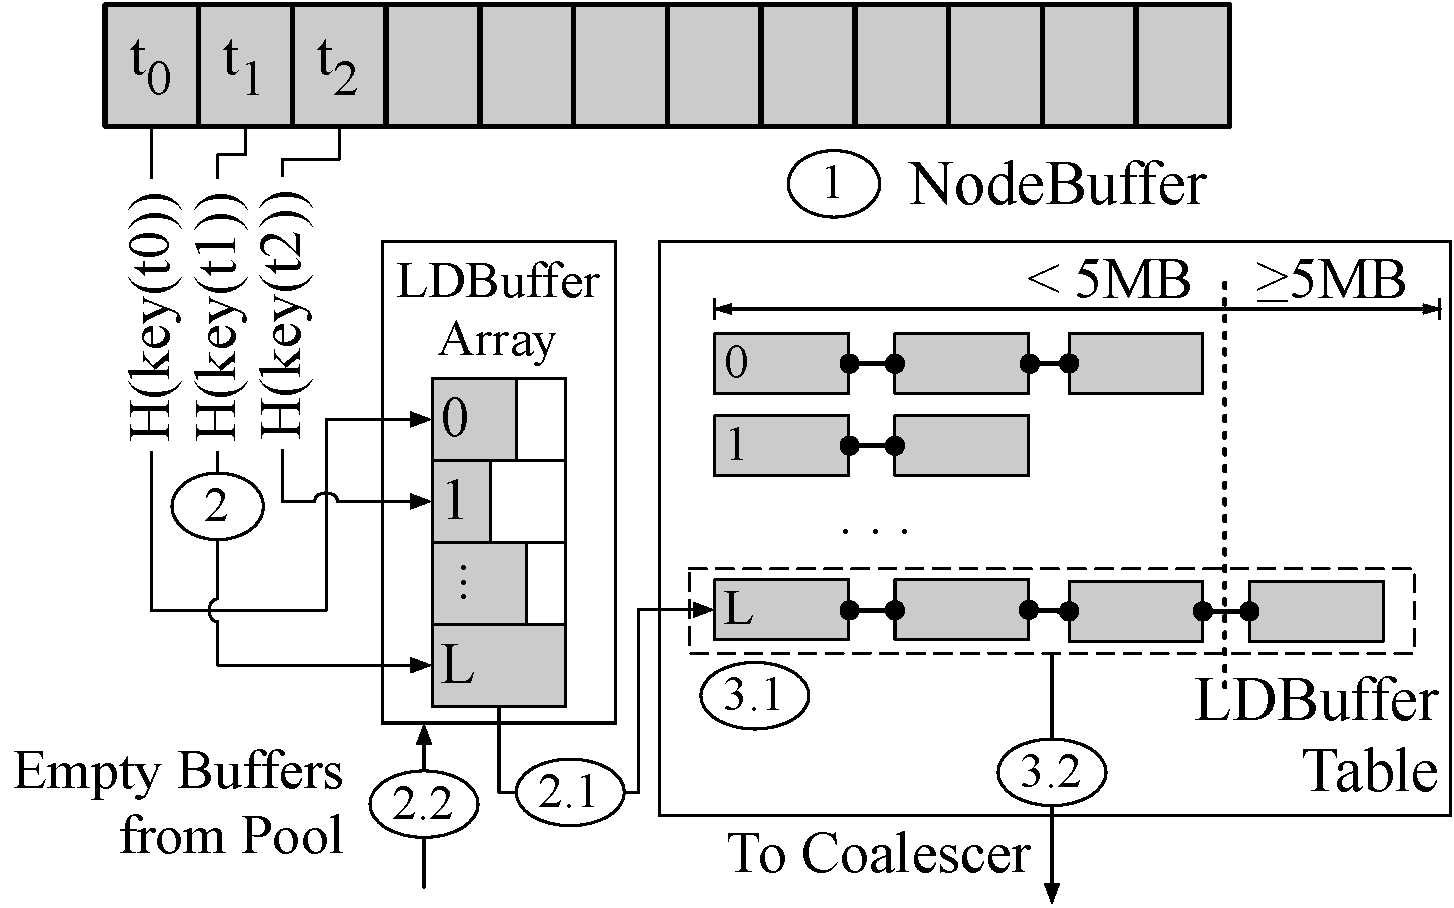
\includegraphics[width=\columnwidth]{tritonsort/figs/ldts_stage.pdf}
  \caption{The \ldts stage, which is responsible for distributing records
  across logical disks and buffering sufficient data to allow for large writes.}
  \label{fig:ldts}
\end{figure}

\paragraph{\ldts:} The \ldts stage, shown in Figure~\ref{fig:ldts}, receives
\nodebuffers from the \receiver that contain records destined for logical disks
on its node.  \ldtss are responsible for distributing records to appropriate
logical disks and sending groups of records destined for the same logical disk to
the downstream \writer stage.

The \ldts's design is driven by the need to buffer enough data to issue large
writes and thereby minimize disk seeks and achieve high bandwidth. Internal to
the \ldts are two data structures: an array of \ldbuffers, one per logical
disk, and an \ldtable.  An \ldbuffer is a buffer of records destined to the same
logical disk.  Each \ldbuffer is 12,800 bytes long, which is the least common
multiple of the record size (100 bytes) and the direct I/O write size (512
bytes).  The \ldtable is an array of \ldbuffer lists, one list per logical disk.
Additionally, \ldts maintains a pool of \ldbuffers, containing 1.25 million
\ldbuffers, accounting for 20 of each machine's 24 GB of memory.

\begin{algorithm}
\begin{algorithmic}[1]
\STATE \nodebuffer $\leftarrow$ getNewWork()\label{alg:ldts:get_work}
\STATE \COMMENT{Drain \nodebuffer into the LDBufferArray}
\FORALL{records $r$ in \nodebuffer}\label{alg:ldts:record_loop_begin}
    \STATE dst $=$ H(key(r))
    \STATE LDBufferArray[dst].append(r)
    \IF{LDBufferArray[dst].isFull()}
        \STATE LDTable.insert(LDBufferArray[dst])
        \STATE LDBufferArray[dst] = getEmptyLDBuffer()
    \ENDIF
\ENDFOR\label{alg:ldts:record_loop_end}

\STATE \COMMENT{Send full LDBufferLists to the Coalescer}
\FORALL{physical disks $d$}\label{alg:ldts:examine_lists_begin}
    \WHILE{LDTable.sizeOfLongestList($d$) $\ge$ 5MB}
        \STATE ld $\leftarrow$ LDTable.getLongestList($d$)
        \STATE \coalescer.pushNewWork(ld)\label{alg:ldts:send_work}
    \ENDWHILE
\ENDFOR\label{alg:ldts:examine_lists_end}
\end{algorithmic}
\caption{The \ldts stage}
\label{alg:ldts}
\end{algorithm}

The operation of a \ldts worker is described in Algorithm~\ref{alg:ldts}. In
Line \ref{alg:ldts:get_work}, a full \nodebuffer is pushed to the \ldts by the
\receiver. Lines \ref{alg:ldts:record_loop_begin}-\ref{alg:ldts:record_loop_end}
are responsible for draining that \nodebuffer record by record into an array of
\ldbuffers, indexed by the logical disk to which the record belongs. Lines
\ref{alg:ldts:examine_lists_begin}-\ref{alg:ldts:examine_lists_end} examine the
\ldtable, looking for logical disk lists that have accumulated enough data to
write out to disk.  We buffer at least 5 MB of data for each logical disk
before flushing that data to disk to prevent many small write requests from
being issued if the pipeline temporarily stalls.  When the minimum threshold of
5 MB is met for any particular physical disk, the longest \ldbuffer list for
that disk is passed to the \coalescer stage on
Line~\ref{alg:ldts:send_work}.

The original design of the \ldts only used the \ldbuffer array described above
and used much larger \ldbuffers (\tilde 10MB each) rather than many small
\ldbuffers. The \coalescer stage (described below) did not exist; instead, the
\ldts transferred the larger \ldbuffers directly to the \writer stage.

This design was abandoned due to its inefficient use of memory. Temporary
imbalances in input distribution could cause \ldbuffers for different logical
disks to fill at different rates.  This, in turn, could cause an \ldbuffer to
become full when many other \ldbuffers in the array are only partially full.
If an \ldbuffer is not available to replace the full buffer, the system must
block (either immediately or when an input record is destined for that buffer's
logical disk) until an \ldbuffer becomes available.  One obvious solution to
this problem is to allow partially full \ldbuffers to be sent to the \writers
at the cost of lower \writer throughput. This scheme introduced the further
problem that the unused portions of the \ldbuffers waiting to be written could
not be used by the \ldts.  In an effort to reduce the amount of memory wasted
in this way, we migrated to the current architecture, which allows small
\ldbuffers to be dynamically reallocated to different logical disks as the need
arises.  This comes at the cost of additional computational overhead and memory
copies, but we deem this cost to be acceptable due to the small cost of memory
copies relative to disk seeks.

\paragraph{\coalescer:} The operation of the \coalescer stage is simple.  A
\coalescer will copy records from each \ldbuffer in its input \ldbuffer list
into a \writerbuffer and pass that \writerbuffer to the \writer stage. It then
returns the \ldbuffers in the list to the \ldbuffer pool.

Originally, the \ldts stage did the work of the \coalescer stage.  While
optimizing the system, however, we realized that the non-trivial amount of time
spent merging \ldbuffers into a single \writerbuffer could be better spent
processing additional \nodebuffers.

\paragraph{\writer:}  The operation of the \writer stage is also quite simple.
When a \coalescer pushes a \writerbuffer to it, the \writer worker will
determine the logical disk corresponding to that \writerbuffer and write out
the data using a blocking \textit{write()} system call.  When the write
completes, the \writerbuffer is returned to the pool.

%\textbf{Possible repeated text.}To ensure maximum utilization of the read/write
%throughput of each disk, we partition the disks on each node into a set of
%input disks and a set of intermediate disks. Further, to reduce contention for
%access to the disks, we assign one \reader worker to every input disk and one
%\writer worker to every intermediate disk. As we show later in our evaluation,
%this setup enables us to balance the operation of the whole system---8 \reader
%workers continuously reading from 8 disks, 8 \writer workers continuously
%writing to 8 other disks, the 10 Gbps network sustaining the data transmitted
%between \sender and \receiver workers, and an appropriate number of \pnts and
%\ldts workers to keep up with the remaining stages.

\subsection{\tritonsort Architecture: Phase Two}

\begin{figure}
  \centering
  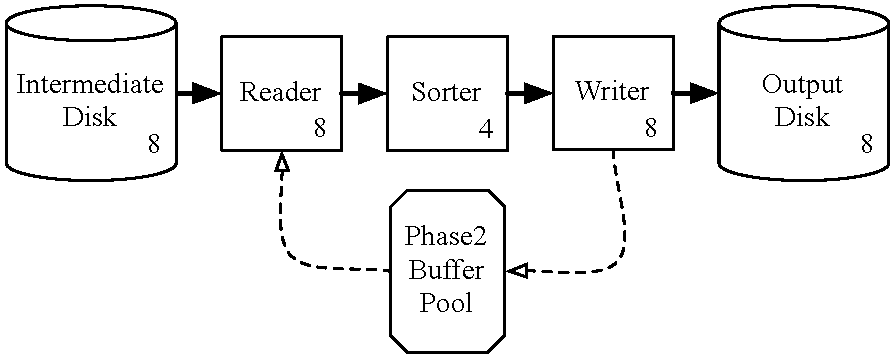
\includegraphics[width=\columnwidth]{tritonsort/figs/phase2.pdf}

  \caption{Block diagram of \tritonsort's phase two architecture.  The
    number of workers for a stage is indicated in the lower-right corner of
    that stage's block, and the number of disks of each type is indicated in
    the lower-right corner of that disk's block.}
  \label{fig:phase2}
\end{figure}

Once phase one completes, all of the records from the input dataset are stored
in appropriate logical disks across the cluster's intermediate disks.  In phase
two, each of these unsorted logical disks is read into memory, sorted, and
written out to an output disk.  The pipeline is straightforward: \reader and
\writer workers issue sequential, streaming I/O requests to the appropriate
disk, and \sorter workers operate entirely in memory.

\paragraph{\reader:}  The phase two \reader stage is identical to
the phase one \reader stage, except that it reads into a \phasetwobuffer, which
is the size of a logical disk.

\paragraph{\sorter:}  The \sorter stage performs an in-memory sort on a
\phasetwobuffer.  A variety of sort algorithms can be used to implement this
stage, however we selected the use of radix sort due to its speed.  Radix sort
requires additional memory overhead compared to an in-place sort like
QuickSort, and so the sizes of our logical disks have to be sized appropriately
so that enough \reader--\sorter--\writer pipelines can operate in parallel.
Our version of radix sort first scans the buffer, constructing a set of
structures containing a pointer to each record's key and a pointer to the record
itself.  These structures are then sorted by key.  Once the structures have
been sorted, they are used to rearrange the records in the buffer in-place. This
reduces the memory overhead for each \sorter substantially at the cost of
additional memory copies.

\paragraph{\writer:}  The phase two \writer writes a \phasetwobuffer
sequentially to a file on an output disk. As in phase one, each \writer is
responsible for writes to a single output disk.

Because the phase two pipeline operates at the granularity of a logical disk,
we can operate several of these pipelines in parallel, limited by either the
number of cores in each system (we can't have more pipelines than cores without
sacrificing performance because the \sorter is CPU-bound), the amount of
memory in the system (each pipeline requires at least three times the size of a
logical disk to be able to read, sort, and write in parallel), or the
throughput of the disks.  In our case, the limiting factor is the
output disk bandwidth.  To host one phase two pipeline per input
disk requires storing 24 logical disks in memory at a time.  To
accomplish this, we set $size_{LD}$ to 850 MB, using most of the 24 GB of RAM
available on each node and allowing for additional memory required by the
operating system.  To sort 850 MB logical disks fast enough to not block the
\reader and \writer stages, we find that four \sorters suffice.

\subsection{Stage and Buffer Sizing}

One of the major requirements for operating \tritonsort at near disk speed is
ensuring cross-stage balance.  Each stage has an intrinsic execution time,
either based on the speed of the device to which it interfaces (e.g., disks or
network links), or based on the amount of CPU time it requires to process a
work unit.  Table~\ref{tbl:stageruntimes} shows the speed and performance of
each stage in the pipeline.  In our implementation, we are limited by the speed
of the \writer stage in both phases one and two.

\begin{table*}
\caption{\label{tbl:stageruntimes}Median stage runtimes for a 52-node,
  100TB sort, excluding the amount of time spent waiting for buffers.}
\centering
\resizebox{\columnwidth}{!}{%
\begin{tabular}{|c|c|c|c|c|c|}
\hline
\textbf{Worker Type} & \textbf{Size Of} & \textbf{Runtime} & \textbf{\# Workers} & \textbf{Throughput} & \textbf{Total Throughput} \\
& \textbf{Input (MB)} & \textbf{(ms)} & & \textbf{(in MBps)} & \textbf{(in MBps)} \\
\hline
\reader    & 81.92 & 958.48 & 8 & 85    & 683 \\
\pnts      & 81.92 & 263.54 & 3 & 310   & 932 \\
%\sender    & 1.65  & 1.38  & 1 & 1188  & 1188 \\
%\receiver  & 1.65  & 1.38  & 1 & 1188  & 1188 \\
\ldts      & 1.65  & 2.42   & 1 & 683   & 683 \\
\coalescer & 10.60  & 4.56   & 8 & 2,324 & 18,593 \\
\writer    & 10.60  & 141.07 & 8 & 75    & 601 \\
\hline
Phase two \reader & 762.95 & 8,238 & 8 & 92 & 740 \\
Phase two \sorter & 762.95 & 2,802 & 4 & 272 & 1089 \\
Phase two \writer & 762.95 & 8,512 & 8 & 89 & 717 \\
\hline
\end{tabular}%
}
\end{table*}

% LocalWords:  enqueueing enqueued dataflow priori getNewWork isFull Coalescer
% LocalWords:  getEmptyLDBuffer LDBufferLists sizeOfLongestList pushNewWork
% LocalWords:  getLongestList dataset QuickSort Runtime runtimes LocalWords
